\documentclass{article}

\usepackage{lmodern}
\usepackage[T1]{fontenc}
\usepackage[spanish,activeacute]{babel}
\usepackage{mathtools}
\usepackage{graphicx}


\title{Pr\'actica 2 }
\author{Mar\'ia de los \'Angeles Rodr\'iguez Vela}

\begin{document}

\maketitle

1. Sea $M=(\{q_0,q_1,\}, \{a,b\}, \delta, q_0, \{q_0\})$ un AFD con:\\

\begin{table}[h!]
\begin{tabular}{c|c|c}
  $\delta(q,\sigma)$ & $a$ & $b$\\
  \hline
  $q_0$& $q_0$ & $q_1$\\
  \hline
  $q_1$& $q_1$ & $q_1$\\
  
\end{tabular}
\end{table}







2.



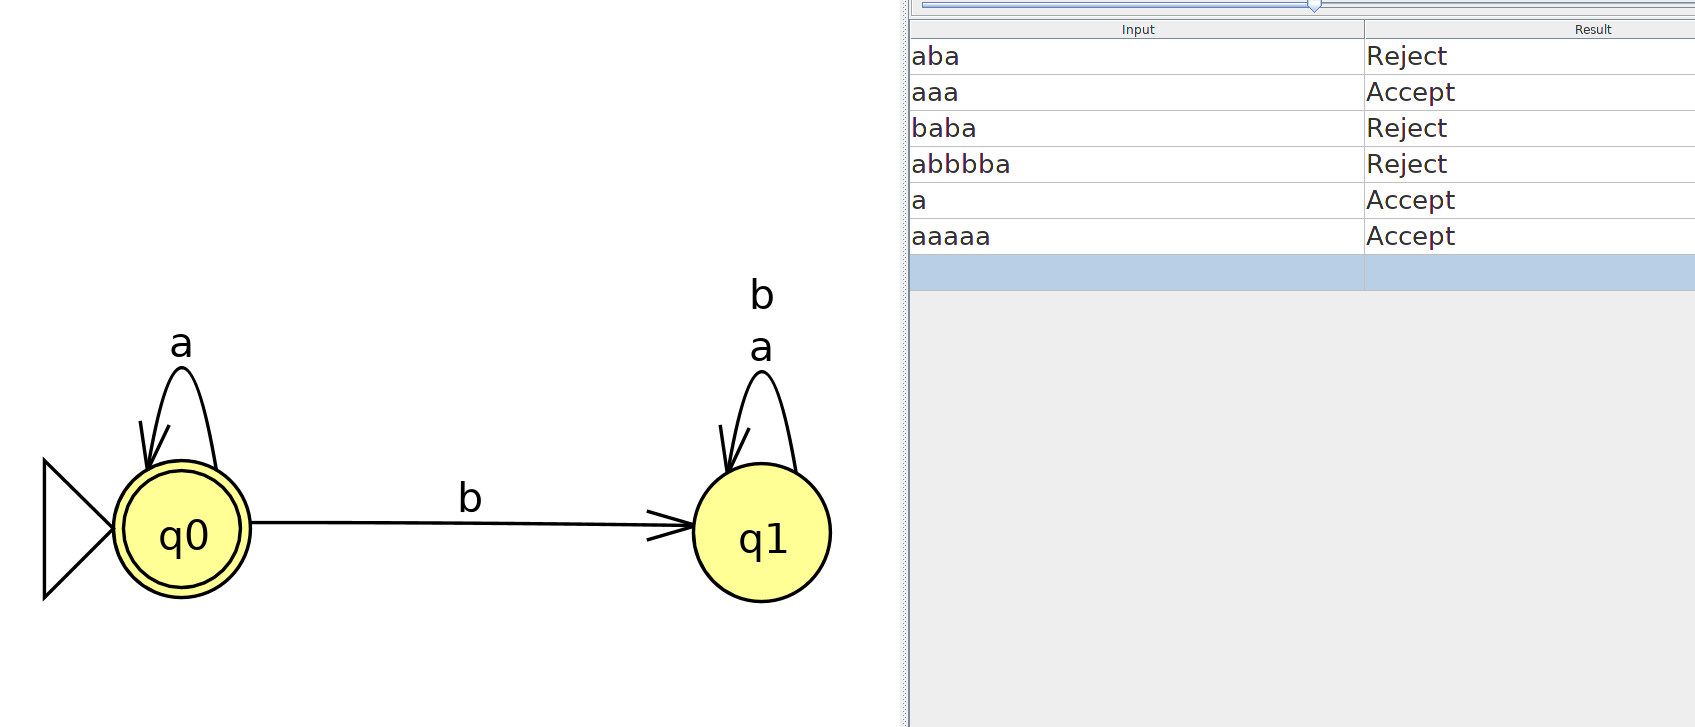
\includegraphics[height=5 cm]{Ejercicio1P2.png}



3.


\begin{verbatim}
[
  {
    "name" : "a",
    "representation" : {
      "K" : ["q0", "q1"],
      "A" : ["a", "b"],
      "s" : "q0",
      "F" : ["q0"],
      "t" : [["q0", "a", "q0"],
             ["q0", "b", "q1"],
             ["q1", "a", "q1"],
             ["q1", "b", "q1"]]
      }
  }
]
\end{verbatim}
\end{document}